\documentclass[aspectratio=169,10pt]{beamer}

\usetheme{metropolis}
\usefonttheme{professionalfonts}
\usepackage{booktabs}
\usepackage{amsmath}
\usepackage{tikz}
\usepackage{qrcode}
\usetikzlibrary{arrows.meta,decorations.pathmorphing,positioning}

\definecolor{Navy}{HTML}{12355B}
\definecolor{Teal}{HTML}{007C7A}
\definecolor{Coral}{HTML}{D95D39}
\definecolor{Gold}{HTML}{D7A500}
\setbeamercolor{normal text}{fg=Navy,bg=white}
\setbeamercolor{alerted text}{fg=Coral}
\setbeamercolor{frametitle}{fg=Navy,bg=white}
\setbeamercolor{progress bar}{fg=Teal,bg=Navy!15}
\setbeamercolor{title separator}{fg=Teal}
\setbeamertemplate{navigation symbols}{}
\setbeamertemplate{footline}{\hfill\insertframenumber\,/\,\inserttotalframenumber\hspace{1em}\vspace{0.7em}}

\title{Spring--Mass--Damper Dynamics}
\subtitle{Equations, variables, and power balance used in the simulation}
\author{Based on \texttt{spring\_mass\_damper.py}}
\date{}

\begin{document}

\maketitle

\begin{frame}{Physical model and sign convention}
\begin{columns}[c]
\column{0.55\textwidth}
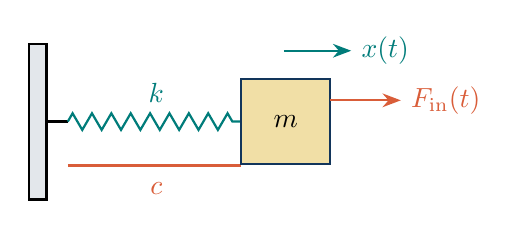
\begin{tikzpicture}[>=Stealth, thick, scale=0.9]
  \draw[fill=Navy!12] (-3,-1.1) rectangle (-2.75,1.1);
  \draw (-2.75,0) -- (-2.45,0);
  \draw[decorate, decoration={zigzag,segment length=7pt,amplitude=3pt}, Teal] (-2.45,0) -- (0,0);
  \draw[Coral, line width=1.2pt] (-2.45,-0.62) -- (0,-0.62);
  \draw[fill=Gold!35, draw=Navy] (0,-0.6) rectangle (1.25,0.6);
  \node at (0.625,0) {$m$};
  \draw[->,Teal] (0.6,1.0) -- (1.55,1.0) node[right] {$x(t)$};
  \draw[->,Coral] (1.25,0.3) -- (2.25,0.3) node[right] {$F_{\mathrm{in}}(t)$};
  \node[Teal] at (-1.2,0.4) {$k$};
  \node[Coral] at (-1.2,-0.95) {$c$};
\end{tikzpicture}
\column{0.42\textwidth}
\begin{block}{Convention used by the script}
Positive displacement and applied force point to the right. Positive power is power delivered \emph{to the mass}.
\end{block}
\vspace{0.4em}
The spring and damper forces exerted on the mass oppose displacement and velocity:
\[
F_s=-kx, \qquad F_d=-c\dot{x}.
\]
\end{columns}
\end{frame}

\begin{frame}{Equation of motion}
\begin{block}{Forced linear model}
\[
\boxed{m\ddot{x}(t)+c\dot{x}(t)+kx(t)=F_{\mathrm{in}}(t)}
\]
\end{block}
\vspace{0.5em}
Newton's second law is evaluated in the code as
\[
\ddot{x}=a=\frac{F_{\mathrm{in}}-c\dot{x}-kx}{m}.
\]
\begin{columns}[T]
\column{0.46\textwidth}
\textbf{Force balance}
\[
F_{\mathrm{net}}=F_{\mathrm{in}}+F_s+F_d=ma.
\]
\column{0.46\textwidth}
\textbf{Free response}\par
When $F_{\mathrm{in}}=0$:
\[
m\ddot{x}+c\dot{x}+kx=0.
\]
\end{columns}
\end{frame}

\begin{frame}{Variables and default values}
\small
\begin{tabular}{@{}lll@{}}
\toprule
Symbol & Meaning & Script default (SI) \\
\midrule
$m$ & Mass & $1.0\ \mathrm{kg}$ \\
$c$ & Viscous damping coefficient & $0.5\ \mathrm{N\,s/m}$ \\
$k$ & Spring stiffness & $10.0\ \mathrm{N/m}$ \\
$x,\;v=\dot{x},\;a=\ddot{x}$ & Displacement, velocity, acceleration & $x(0)=0,\;v(0)=0$ \\
$t$ & Simulation time & $0\leq t\leq20\ \mathrm{s}$ \\
$F_{\mathrm{in}}$ & Externally applied force & pulse amplitude $k x_{\mathrm{target}}$ \\
$x_{\mathrm{target}}$ & Pulse target displacement & $0.05\ \mathrm{m}$ \\
$t_p$ & Pulse duration & $1.0\ \mathrm{s}$ \\
\bottomrule
\end{tabular}
\vspace{1em}
\begin{alertblock}{Input used in the script}
\[
F_{\mathrm{in}}(t)=
\begin{cases}
kx_{\mathrm{target}}, & t\leq t_p,\\
0, & t>t_p.
\end{cases}
\qquad\Rightarrow\qquad F_{\mathrm{in}}=0.5\ \mathrm{N}\ \text{during the pulse.}
\]
\end{alertblock}
\end{frame}

\begin{frame}{First-order state representation}
The ODE solver advances the state vector
\[
\mathbf{z}=\begin{bmatrix}x\\v\end{bmatrix},
\qquad
\dot{\mathbf{z}}=
\begin{bmatrix}
\dot{x}\\\dot{v}
\end{bmatrix}
=
\begin{bmatrix}
v\\[0.25em]
\dfrac{F_{\mathrm{in}}-cv-kx}{m}
\end{bmatrix}.
\]
\vspace{0.6em}
Equivalently,
\[
\dot{\mathbf{z}}=
\underbrace{\begin{bmatrix}0&1\\-k/m&-c/m\end{bmatrix}}_{A}\mathbf{z}
+
\underbrace{\begin{bmatrix}0\\1/m\end{bmatrix}}_{B}F_{\mathrm{in}}.
\]
\begin{block}{Numerics}
The script uses \texttt{scipy.integrate.solve\_ivp} with RK45 at $100001$ sampled time points, $rtol=10^{-9}$, and $atol=10^{-11}$.
\end{block}
\end{frame}

\begin{frame}{Instantaneous power}
For a force acting on the mass, $P=Fv$. The implementation therefore calculates:
\[
\begin{aligned}
P_{\mathrm{spring}} &= F_s v=-kxv,\\
P_{\mathrm{damper}} &= F_d v=-cv^2\leq0,\\
P_{\mathrm{input}} &= F_{\mathrm{in}}v,\\
P_{\mathrm{net}} &= F_{\mathrm{net}}v=mav=\frac{dK}{dt}.
\end{aligned}
\]
\vspace{0.5em}
\begin{columns}[T]
\column{0.47\textwidth}
\begin{block}{Damper loss rate}
\[
P_{\mathrm{dissipated}}=-P_{\mathrm{damper}}=cv^2\geq0.
\]
\end{block}
\column{0.47\textwidth}
\begin{block}{Code convention}
A negative component power means that component removes energy from the mass.
\end{block}
\end{columns}
\end{frame}

\begin{frame}{Stored energy and balance}
\begin{columns}[T]
\column{0.48\textwidth}
\textbf{Energy definitions}
\[
K=\tfrac12mv^2,\qquad U=\tfrac12kx^2,
\]
\[
E_{\mathrm{mech}}=K+U.
\]
Their rates are
\[
\frac{dK}{dt}=mav,\qquad \frac{dU}{dt}=kxv.
\]
\column{0.48\textwidth}
\textbf{Power balance}
\[
\frac{dE_{\mathrm{mech}}}{dt}
=\frac{dK}{dt}+\frac{dU}{dt}
=P_{\mathrm{input}}+P_{\mathrm{damper}}.
\]
Because $P_{\mathrm{damper}}\leq0$, damping drains mechanical energy.
\end{columns}
\vspace{0.6em}
\begin{alertblock}{Integrated balance checked by the script}
\[
E_{\mathrm{mech}}(t)+E_{\mathrm{diss}}(t)
=E_{\mathrm{mech}}(0)+E_{\mathrm{input}}(t),
\]
where $E_{\mathrm{diss}}=\int_0^t cv^2\,d\tau$ and $E_{\mathrm{input}}=\int_0^t F_{\mathrm{in}}v\,d\tau$.
\end{alertblock}
\end{frame}

\begin{frame}{Active and reactive mechanical power}
\begin{block}{Mechanical analogy used in the script}
\[
\boxed{P_{\mathrm{active}}=P_{\mathrm{dissipated}}=cv^2}
\qquad
\boxed{P_{\mathrm{reactive}}=\frac{dU}{dt}+\frac{dK}{dt}}
\]
\end{block}
\vspace{0.4em}
\begin{itemize}
\item The damper is resistive: it irreversibly converts mechanical energy to heat.
\item The spring and mass are storage elements: their energy changes reversibly between $U$ and $K$.
\item The script plots both quantities alongside instantaneous input power and stored/dissipated energy.
\end{itemize}
\end{frame}

\begin{frame}{Key response properties}
\begin{columns}[c]
\column{0.52\textwidth}
\[
\omega_n=\sqrt{\frac{k}{m}},\qquad
c_{\mathrm{crit}}=2\sqrt{km},\qquad
\zeta=\frac{c}{c_{\mathrm{crit}}}.
\]
For $\zeta<1$:
\[
\omega_d=\omega_n\sqrt{1-\zeta^2}.
\]
\column{0.42\textwidth}
\begin{block}{Defaults evaluated}
\begin{align*}
\omega_n &= 3.1623\ \mathrm{rad/s},\\
c_{\mathrm{crit}} &= 6.3246\ \mathrm{N\,s/m},\\
\zeta &= 0.0791.
\end{align*}
\centering\alert{Underdamped response}
\end{block}
\end{columns}
\vfill
\centering
\Large The pulse injects energy; the spring and mass exchange it; the damper dissipates it.
\end{frame}

\begin{frame}{Explore the interactive simulation}
\begin{columns}[c]
\column{0.55\textwidth}
\Large
Adjust the model parameters and inspect the response, forces, power, and energy in the live Streamlit app.

\vspace{1.2em}
\normalsize
\href{https://springmassdamperurp.streamlit.app/}{\color{Teal}\texttt{springmassdamperurp.streamlit.app}}

\vspace{0.8em}
\small Scan the QR code or follow the link to open the simulation.

\column{0.35\textwidth}
\centering
\qrcode[height=3.4cm]{https://springmassdamperurp.streamlit.app/}
\end{columns}
\end{frame}



\end{document}
